\section{Odometry}

In last years driverless pipeline the state estimation algorithm was one of the weak points. It had too much drift and was very susceptible to slip. A new, more complete method was therefore needed. The first few months of the authors time in Revolve were therefore spent looking into different methods.

The team was overall very fond of the idea of single sensor odometry sources like visual odometry or LiDAR odometry. If these could be made to work well it would mean having an odometry source for our test trolley, which in turn would mean not having to wait for the car to be finished to test our full autonomous pipeline. A handful of these were therefore tried out. However, these all turned out to be very unstable. This is thought to come from the fact that the track consists of only uniform tarmac and cones. The track therefore did not give the algorithms enough features to compare, leading to bad performance.

Other approaches to state estimation were then looked into. After discussions with alumni from last year it was decided that ease of tuning was to be an important point, since test time was believed to be scarce. This lead the author to search beyond the EKF, as this has a lot of tuning parameters and needs to be linearized around several points with a separate set of tuning gains for each linearization points. 

A nonlinear observer was therefore thought to be promising, and after some literature studies it was discovered that very similar problems to ours had been solved previously here at NTNU. 

\subsection{Summary of odometry design}

Following the work done in ref \cite{Automatica08} and ref \cite{MainStateEst}, it was decided to implement a nonlinear observer, estimating longitudinal and lateral velocity, yaw rate, ground-tyre friction coefficient, bank angle and inclination angle.

The observer has two modes; one where it updates the estimate of all the states except the friction coefficient, and one where it updates all but the estimate of bank angle. This is because the way they are estimated makes renders them unobservable at the same time. 
The main idea behind the entire observer is to approximate when different sources of information are to be trusted more than others. The conflict is usually between \gls{IMU} data and estimates calculated from the state estimates and measurements of the angles and \glspl{RPM} of the wheels.

\subsection{Nonlinear observer design}

The design of this observer is explained below, by first talking about each state separately, before discussing the full estimator.

\subsubsection{Longitudinal velocity}
For the longitudinal velocity there are three sources of information; the rotational speed of the wheels, the acceleration measured by the \gls{IMU} and the power used by the motors. It was decided to use the former two. Using the power from the motor might have given a better estimate of the slip ratio, but it was deemed to complex and time consuming for the allotted time. 

To estimate the longitudinal velocity the following observer was used
\begin{equation}
    \dot{\hat{v}}_x = a_x + \dot{\psi}\hat{v}_y + K_{v_x}(t)(v_{x,rpm} - \hat{v}_x)
\end{equation}
where $\hat{v}_x$ is our estimate of longitudinal velocity $v_x$, $a_x$ is the measured longitudinal acceleration from the IMU, $\dot{\psi}$ is our estimate of the rate of change of the yaw angle and $K_{v_x}(t)$ is a time varying gain, chosen to downweight the velocity calculated from the wheel \glspl{RPM} when the estimates have a high variance. $v_{x,rpm}$ is calculated as 
\begin{equation}
    v_{x,rpm} = mean(\sum_{i=1}^{4} \omega_{i}R_{eff,i}(t))
\end{equation}
where $\omega_i$ is the angular velocity of wheel $i$ and $R_{eff,i}(t)$ is the effective wheel radius of wheel $i$ at time $t$. The wheel radius is a function of ride height only, as the expansion of the tyre due to an increase in rotational speed was deemed negligible. The wheel radius of wheel $i$ is calculated using the so called Magic Formula 5.2 for the tire radius \cite{MagicFormula5_2}

\begin{equation}
    R_{eff,i}(t) = R_0 - (R_0-R_{L800N}([D_{R_{eff}}atan(B_{R_{eff}}\rho) + \\ F_{R_{eff}}\rho]
\end{equation}
with
\begin{equation}
    \rho = \frac{R_0-R_l(t)}{R_0-R_{L800N}}
\end{equation}

The coefficients $D_{R_{eff}}, B_{R_{eff}}$ and $F_{R_{eff}}$ where in the tyres data sheet, and $R_0$ and $R_{L800N}$ where found empirically. $R_0$ is the radius when unloaded, while $R_{L800N}$ is the radius of the wheel when loaded with 800N, averaged over measurements in different angles. $R_l(t)$ is the current distance from the wheel centre to the ground, either measured by a ride height sensor, or estimated using estimates of the wheel loads.

\subsubsection{Lateral velocity} 
To estimate the lateral velocity, an estimate of the lateral forces is first made, by using the pure lateral magic formula 5.2 \cite{MagicFormula5_2}. This assumes that the longitudinal acceleration is negligible, but since the controller is told to never accelerate in corners, this assumption should be satisfied when it matters. The only time when the controller does accelerate when cornering is when the emergency brake has been turned on, in which case the state estimation isn't going to be used anyways and the whole system needs to be rebooted. 

The magic formula gives the lateral force on each wheel in the wheel frame. These are then rotated into the body-fixed frame located in the \gls{CG}, and summed to find the total lateral acceleration. This is done by doing the following calculation

\begin{align}
    F_y(F_{z,i},\hat{v_x},\hat{v_y},\dot{\hat{\psi}}, \theta) & = \frac{1}{\mu_{H}^{*}}\sum_{i=1}^{4}cos(\delta_i)\theta F_{y,i}(F_{z,i},\hat{v_x},\hat{v_y},\dot{\hat{\psi}}, \mu_{H}^{*}) \\
    & =  \theta F_y^{*}
\end{align}

$F_{y,i}(F_{z,i},\hat{v_x},\hat{v_y},\dot{\hat{\psi}}, \mu_{H}^{*})$ is the lateral force on wheel $i$ at the nominal value of the friction coefficient $\mu_{H}^{*}$. $\theta$ is the estimate of the friction coefficient. $F_{z,i}$ is the estimated vertical load on wheel $i$. $\delta_i$ is the angle of wheel $i$ with the x-axis of the body frame, found by using a lookup table from the measured steering wheel angle to the wheel angle. Note that for the two rear wheels the wheel angle $\delta_i$ is always zero. 

$F_{z,i}$ is found by adding together the force on the wheel when the car is standing still, with the shifted weight found by using the lateral and longitudinal acceleration measurements.  

The above calculation gives the lateral force, which is then divided by $(1 + p_{\phi}g)m$ to give the pure lateral acceleration. $g$ is the gravitational constant at sea level, $m$ is the mass of the vehicle and $p_{\phi}$ is the so called roll gradient, giving the relationship between the lateral acceleration and roll angle. This removes the added acceleration in the lateral direction as a result of roll angle when cornering. Calling this new acceleration estimate $a_y = \theta a_y^*$. This estimate is then used in the observer for the lateral velocity

\begin{equation}
    \dot{\hat{v}}_y = a_y - \dot{\hat{\psi}}\hat{v}_x + K_{v_y}\xi(t,\hat{x})\Lambda(a_y - \theta a_y^{*}) + \frac{\Gamma_2}{\Gamma_1}\zeta(\dot{\psi} - \dot{\hat{\psi}})
\end{equation}

where $\Gamma_1$ and $\Gamma_2$ are positive gain and $\xi(t,\hat{x})$ is a time varying gain that gives how much faith is put in the magic formula estimated acceleration compared with the one from the \gls{IMU}. Following the discussion in \cite{MainStateEst} and \cite{FossenGrip2007}, this was chosen to be

\begin{equation}
    \xi(t,\hat{x}) = \frac{\delta \hat{a}_y^*}{\delta \hat{v}_y}(t,\hat{x})
\end{equation}

The idea is that this value for $\xi$ will be approximately the slope of the line between $(\hat{v}_y,\hat{a}_y^*(t,\hat{v}_v,\hat{v}_y))$ and $v_y,\hat{a}_y^*(t,\hat{v}_x,v_y))$, which is needed to get the time derivative of Lyapunov function defined in \cite{FossenGrip2007} to be negative definite.

$\Lambda$ is a scaling signal that prevents large variations in the gain. This was chosen to be

\begin{equation}
    \Lambda(t,\hat{x}) = (\xi^2(t,\hat{x}) + \hat{a}_y^2(t,\hat{x}))^{-1/2}
\end{equation}

Similarly $\zeta$ is a gain that determines how much faith is put in the yaw rate estimate determined by the wheel velocities versus the yaw rate measurement coming out of the IMU.

\subsubsection{Yaw rate}

To estimate the yaw rate, the \gls{IMU} provides a estimate of the yaw rate, but since this is noisy it is desirable to add one more source of information. To do this the magic formula for the lateral force on the wheels is uses, but this time use it to find the torque around the CG

\begin{equation}
    f_r(F_{z,i}, \hat{v_x}, \hat{v_y}, \dot{\hat{\psi}}) =\theta f_r^*(F_{z,i}, \hat{v_x}, \hat{v_y}, \dot{\hat{\psi}}) 
\end{equation}
where
\begin{equation}
    f_r^*(F_{z,i}, \hat{v_x}, \hat{v_y}, \dot{\hat{\psi}}) = \frac{1}{\mu_H^*}\sum_{i=1}^{4}g_i^TR(\delta_i)F_{y,i}(F_{z,i}, \hat{v_x}, \hat{v_y}, \dot{\hat{\psi}}, \mu_H^*)
\end{equation}
with 

\begin{equation}
    g_i = \begin{bmatrix} -l_i sin(\alpha_i) \\ h_i cos(\alpha_i)
    \end{bmatrix}
\end{equation}
where for convenience it has been defined

\begin{align}
    \alpha_1 & = -\gamma_1 \\
    \alpha_2 & = \gamma_2 \\
    \alpha_3 & = \pi + \gamma_3 \\
    \alpha_4 & = \pi -\gamma_4 \\
\end{align}

The $l_i$ is the length from the \gls{CG} to wheel $i$, while $\gamma_i$ is the angle the line going through both CG and wheel $i$ make with the longitudinal axis of the car. This is more easily understood by looking at figure \ref{Fig:WheelTorques}. 

\begin{figure}
    \centering
    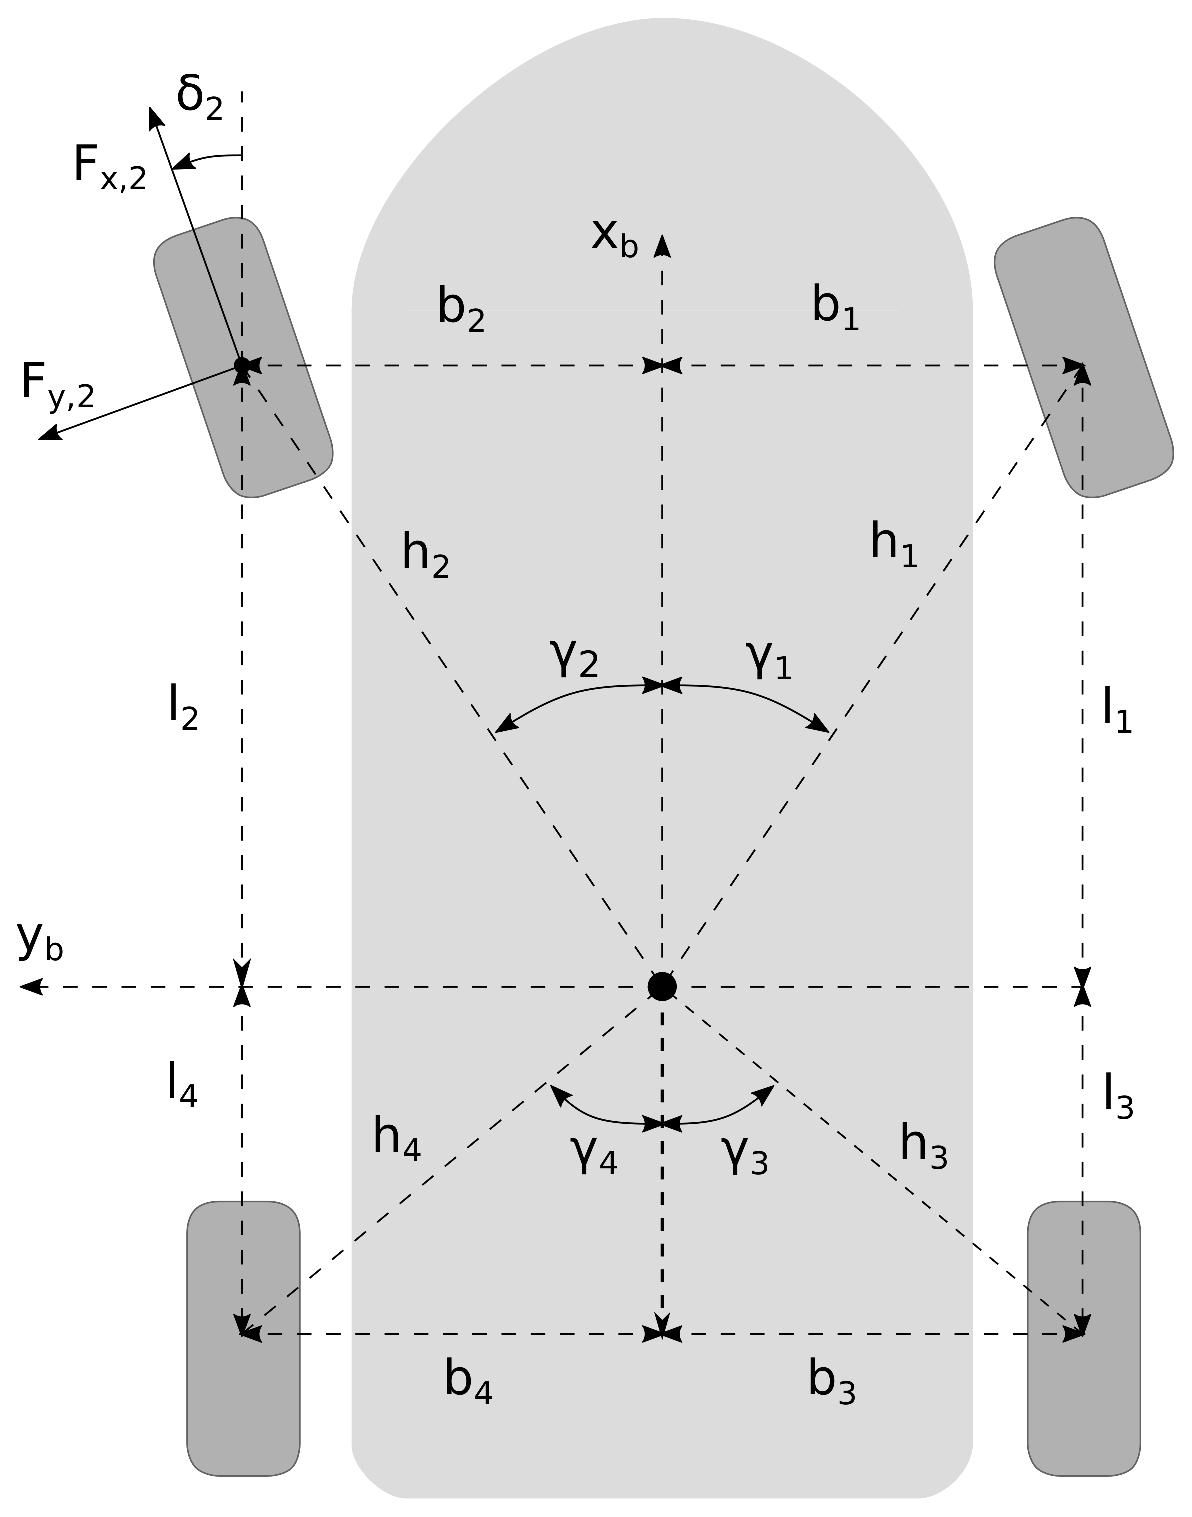
\includegraphics[width=0.5\linewidth]{0_Images/3_Theory/TorqueCalculations.eps}
    \captionof{figure}{Illustrations of variables used for torque calculations.}
    \label{Fig:WheelTorques}
\end{figure}

This estimate is then used in much the same way as for the longitudinal velocity to update the estimate of the yaw rate,

\begin{equation}
    \ddot{\hat{\psi}} = \frac{1}{J}\theta \hat{f}_r^* + k_r(\dot{\psi}-\hat{\dot{\psi}})
\end{equation}

where $J$ is the moment of inertia of the vehicle around CG, and $K_r$ is how much faith is put in the estimate calculated by looking at lateral tyre forces, compared to yaw rate coming out of the IMU. 

\subsubsection{Friction parameter}
Instead of estimating the friction parameter directly, which would have meant one friction coefficient per wheel, the lateral force is parametrised as earlier

\begin{equation}
    f_y(F_{z,i}, \hat{v_x}, \hat{v_y}, \dot{\hat{\psi}}) =\theta f_y^*(F_{z,i}, \hat{v_x}, \hat{v_y}, \dot{\hat{\psi}}) 
\end{equation}

This is an acceptable simplification, since the formula student track is uniform tarmac without any oil spill or similar. It will only ever change friction coefficient as a result of weather, and then it is reasonable to assume it is going to affect the track evenly since no parts are going to be under a roof. 

The estimate for the simplified friction coefficient is updated using the following observer

\begin{equation}
    \dot{\theta} = K_{\theta}\Lambda (t, \hat{x})\hat{a}_y^*(t,\hat{x})(a_y - \hat{a}_y(t,\hat{x},\theta))
\end{equation}

\subsubsection{Bank and inclination angle}

The final part of the puzzle is estimating the bank and inclination angle so their effect on the lateral and longitudinal forces can be corrected for. The tilt of the ground is defined as first an inclination angle $\Theta$ around the vehicles y-axis, and then a bank angle $\Phi$ around the now rotated x-axis. This leads to the following effect on the dynamics of the car

\begin{align}
    \dot{v}_x & = a_x + \dot{\psi} v_y + g sin(\Theta) \\
    \dot{v}_y & = a_y - \dot{\psi}v_x - g cos(\Theta) sin(\Phi)
\end{align}

Define $\theta_i = sin(\Theta)$ and $\theta_b = cos(\Theta)sin(\Phi)$. When the bank and inclination angles are small, these are approximately 

\begin{align}
    \theta_i & \approx \Theta \\
    \theta_b & \approx \Phi
\end{align}

Therefore an estimate of $\theta_i$ and $\theta_b$ is introduced by

\begin{align}
    \dot{\hat{\theta}}_i & = K_{\theta_i}K_{v_x}(t)(v_{x,rpm} - \hat{v}_x) \\
    \dot{\hat{\theta}}_b & = K_{\theta_b}(a_y-\hat{a}_y(t,\hat{x},\theta)
\end{align}

where $K_{v_X}$ is, as previously defined, how much faith is put in the longitudinal velocity estimate coming from the wheel \glspl{RPM}. $K_{\theta_i}$ and $K_{\theta_b}$ are tuning parameters. The observers for $v_y$ and $v_x$ are modified to correct for this bias by adding $g\hat{\theta}_i$ to $\dot{\hat{v}}_x$ and $-g\hat{\theta}_b$ to $\dot{\hat{v}}_y$. 

\subsubsection{When to estimate friction}

Estimating the bank angle and estimating the friction coefficient $\theta$ are conflicting problems, as both are not properly observable at the same time. In \cite{MainStateEst} this is solved by turning off the friction coefficient update when there isn't enough lateral acceleration for it to converge properly, and turning off the bank angle update when estimating updating the friction coefficient. They found that this worked well in most cases, but that when driving in terrain that is both hilly, meaning varying bank angle, and with a low friction coefficient, they needed to estimate both at the same time. 

To do this they developed a rather complex set of rules for when to turn on and off the two different update laws. We believe this is not needed in our case, since we are driving on flat ground with a slowly varying bank angle and a friction coefficient that never goes down as low as theirs did. They were driving on snow and ice, while the worst condition we will faced with will be wet tarmac. Therefore, as long as we switch between the two update laws regularly, there shouldn't be a need to estimate both bank angle and friction coefficient at the same time. 

For this reason we employ the same switching rule for when to update the friction coefficient as \cite{MainStateEst} and simply turn off the bank angle update when friction coefficient is being updated. To determine when to turn on the friction update we estimate the reference yaw rate found by looking at the wheel torques, and an estimate of $\dot{v}_y$, called $\dot{\hat{v}}_y$, found by low pass filtering $a_y - \dot{\psi}\hat{v}_x$. A high value for $\dot{\hat{v}}_y$ indicates a high level of excitation and that some of the tyres might be in the nonlinear region where it's possible to get information about the friction coefficient. When both these values are high enough we turn on friction update and turn off bank angle update. 

Ref. \cite{MainStateEst} lets the friction coefficient go exponentially to a nominal value of 1 when it is not being estimated from the sensor data. They argue that dry tarmac will be the normal operating conditions. We chose instead to simply let the coefficient stay at that value when we aren't updating it from the sensor data, arguing that the ground conditions will change rather slowly.

\subsubsection{Final observer}
The full observer has to modes: either it updates the estimate of the bank angle, or it updates the estimate of the friction coefficient. In the first case the full observer is as follows

\begin{align}
    \dot{\hat{v}}_x & = a_x + \dot{\hat{\psi}}\hat{v}_y + g\hat{\theta}_i + K_{v_x}(t)(v_{x,rpm} - \hat{v}_x) \\
    \dot{\hat{v}}_y & = a_y - \dot{\hat{\psi}}\hat{v}_x - g\hat{\theta}_b + K_{v_y}\xi(t,\hat{x})\Lambda(a_y - \theta a_y^{*}) + \frac{\Gamma_2}{\Gamma_1}\zeta(\dot{\psi} - \dot{\hat{\psi}}) \\ 
    \dot{\hat{\theta}}_i & = K_{\theta_i}K_{v_x}(t)(v_{x,rpm} - \hat{v}_x) \\
    \dot{\hat{\theta}}_b & = K_{\theta_b}(a_y-\hat{a}_y(t,\hat{x},\theta)) \\ 
    \ddot{\hat{\psi}} & = \frac{1}{J}\theta \hat{f}_r^* + k_r(t)(\dot{\psi}-\hat{\dot{\psi}})
\end{align}

In the second case, i.e. when updating friction coefficient and not bank angle, the observer uses the following update laws

\begin{align}
    \dot{\hat{v}}_x & = a_x + \dot{\psi}\hat{v}_y + g\hat{\theta}_i + K_{v_x}(t)(v_{x,rpm} - \hat{v}_x) \\
    \dot{\hat{v}}_y & = a_y - \dot{\hat{\psi}}\hat{v}_x - g\hat{\theta}_b + K_{v_y}\xi(t,\hat{x})\Lambda(a_y - \theta a_y^{*}) + \frac{\Gamma_2}{\Gamma_1}\zeta(\dot{\psi} - \dot{\hat{\psi}}) \\ 
    \dot{\hat{\theta}}_i & = K_{\theta_i}K_{v_x}(t)(v_{x,rpm} - \hat{v}_x) \\
    \dot{\theta} & = K_{\theta}\Lambda (t, \hat{x})\hat{a}_y^*(t,\hat{x})(a_y - \hat{a}_y(t,\hat{x},\theta)) \\ 
    \ddot{\hat{\psi}} & = \frac{1}{J}\theta \hat{f}_r^* + k_r(t)(\dot{\psi}-\hat{\dot{\psi}})
\end{align}

\gls{UGAS} and \gls{ULES} of the error of the estimator for $(v_x,v_y,r,\theta)$ was proven in \cite{Automatica08}, while \gls{UGAS} of the error for the estimator for $(v_x,v_y,\theta, \theta_i, \theta_b)$ was proven in \cite{MainStateEst}. The first of these implies \gls{UGAS} and \gls{ULES} of the full observer of $(v_x,v_y, r,\theta, \theta_i, \theta_b)$, as long as the gains on the bank and inclination angle estimates are small enough, and the estimates of $\theta$, $\theta_i$ and $\theta_b$ are limited to a small enough range. This is because \gls{UGAS} together with \gls{ULES} implies a robustness to small constant biases, which is the effect a wrong estimate of the bank and inclination angles would add to the update laws for $\hat{v}_x$ and $\hat{v}_y$. 
